\documentclass[11pt,answers]{exam}

% Load useful packages
% Read in necessary packages
\usepackage{import}
\usepackage{amsmath}
\usepackage{amsfonts}
\usepackage{amssymb}
\usepackage{graphicx}
\usepackage[urlcolor=blue]{hyperref}
\usepackage{color}
\usepackage{subfigure}
\usepackage{tikz}

% Set various options for exam package
\shadedsolutions % defines the style of the solution environment

% Set lesson name, etc.
\newcommand{\coursename}{Math 312}
\newcommand{\lessonname}{Problem Set 3}
\newcommand{\duedate}{9 February 2016}
\newcommand{\names}{Jinqiao Lin, Emily Sanford, Ian Gallmeister}

\title{Homework 3}
% Set headers/footers to look nice
\pagestyle{headandfoot}
\firstpageheader{\textbf{\large \coursename\ \lessonname}}{}{\textbf{\large Due \duedate}}
\firstpageheadrule
\runningheader{\textbf{\large \coursename\ \lessonname}}{}{\textbf{\large Due \duedate}}
\runningheadrule
\firstpagefooter{\names}{}{Page \thepage\ of \numpages}
\firstpagefootrule
\runningfooter{\names}{}{Page \thepage\ of \numpages}
\runningfootrule

% Define commands related to marking up content
\newcommand{\source}[1]{}

% Define commands related to general mathematical style
\renewcommand{\exp}[1]{e^{#1}}

\renewcommand{\theenumi}{(\alph{enumi})}
\renewcommand{\labelenumi}{\theenumi}
\renewcommand{\thequestion}{\arabic{question}}
\renewcommand{\questionlabel}{(\thequestion)}
%%%%%%%%%%%%%%%%%%%%%%%%%%%%%%%%%%%%%%%%%%%%%%%%%%%%%%%%%%%%

\begin{document}
\begin{questions}

\addtocounter{question}{15}

\item We take a Hookean spring with spring constant $3.6 kg/s^2$ and attach a $0.1 kg$ mass to the end of the spring. The spring’s resting position is called $x = 0$. Then we give the mass a sharp tap, imparting an instantaneous rightward velocity of 0.4 m/s. Assuming that there is no damping present, find a formula for the spring displacement as a function of time, $x(t)$. Then state the amplitude and (angular) frequency of the resulting motion. Plot the solution.

\begin{solution}
\newline For this problem, we use Newton’s Law of Forces, where the sum of the forces acting on an object are equal to the mass times the acceleration of the object. We use $\ddot{x}$ for acceleration, since acceleration is the second derivative of position, $x$.

\begin{equation}
m \ddot{x} = -k x - \delta \dot{x} + f(t)
\end{equation}

$kx$ is the spring force, and $k > 0$ because when the displacement is in the negative direction, this force will restore it by moving it in the positive direction, whereas when the displacement is in the positive direction, this force will restore it toward its original position by moving it in the negative direction. $\delta \dot{x}$ is the frictional damping force, with $\delta$ being a positive constant such that the term $-\delta \dot{x}$ is negatively proportional to the velocity. 
$f(t)$ is the external force on the object.

In this situation, $k = 3.6 kg/s^{2}$, $m = 0.1 kg$, $\delta \dot{x} = 0$, and $f(t) = 0$ since there are no frictional damping or external forces. Substituting these values gives us 

\begin{equation}
0.1 \ddot{x} = -3.6 x
\end{equation}

Simplifying this equation gives us a second order differential equation in terms of x.

\begin{equation}
\ddot{x} = \frac{-3.6}{0.1} x = -36 x
\end{equation}

We can solve this homogeneous linear ODE using its characteristic equation, $\lambda^{2} + 36\lambda = 0$, which gives us the roots $\lambda = \pm 6i$. We construct the General Solution for $x(t)$ using these roots:

\begin{equation}
x(t) = C_{1}e^{6it} + C_{2}e^{-6it}
\end{equation}

We then substitute into this equation using Euler’s formulas, $e^{i\theta} = \cos{(\theta)} + i\sin{(\theta)}$ and $e^{-i\theta} = \cos{(\theta)} - i\sin{(\theta)}$. This gives us the following:

\begin{equation}
x(t) = C_{1}(\cos{(6t)} + i\sin{(6t)}) + C_{2}(\cos{(6t)} – i\sin{(6t)})
\end{equation}

This simplifies to

\begin{equation}
x(t) = (C_{1} + C_{2}) (\cos{(6t)}) + (C_{1} - C_{2}) (i\sin{(6t)})
\end{equation}

Let $C_{3} = C_{1} + C_{2}$ and $C_{4} = C_{1} - C_{2}$ (since they are all constants) and simplify again to get a new general solution for the position function, this time in terms of sine and cosine.

\begin{equation}
x(t) = C_{3} \cos{(6t)} + C_{4} i \sin{(6t)}
\end{equation}

We can use our initial condition $x_{0} = 0$ to solve for $C_{3}$.

\begin{equation}
x(0) = 0 = C_{3} \cos{(0)} + C_{4} i \sin{(0)}
\end{equation}

Since $\sin{(0)} = 0$ and $\cos{(0)}$ = 1, $C_{3} = 0$.

Now we can find a formula for $\dot{x}(t)$ by differentiating our new general solution.

\begin{equation}
\dot{x}(t) = 6 C_{4} i \cos{(6t)}
\end{equation}

Now we use our initial condition, $v_{0} = \dot{x}_{0} = 0.4 m/s$.

\begin{equation}
\dot{x}(0) = 0.4 = 6 C_{4} i \cos{(0)}
\end{equation}

Since $\cos{(0)} = 1$,

\begin{equation}
0.4 = 6 C_{4} i 
\end{equation}

We solve this equation for $c_{4}$ and find $c_{4} = \frac{1}{15i}$. 

This gives us the following particular solution for $x(t)$:

\begin{equation}
x(t) = \frac{1}{15i} i \sin{(6t)} = \frac{1}{15} \sin{(6t)}
\end{equation}

This equation for the position $x$ of the mass is periodic, with an angular frequency of $\frac{6}{2 \pi} = \frac{3}{\pi}$ and an amplitude of $\frac{1}{15}$. 
 

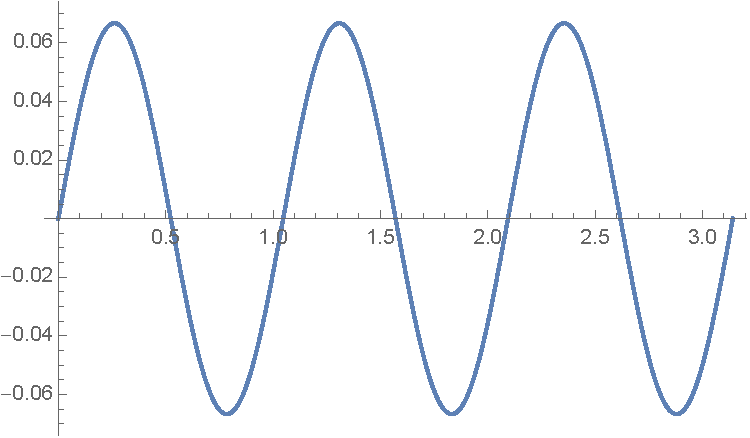
\includegraphics{p16plot.pdf}
\end{solution}

\pagebreak

\item We take a Hookean spring with spring constant $9.8$ $kg/s^2$ and attach a $0.1$ $kg$ mass to the end of the spring. The spring’s resting position is called $x = 0$. The system is placed in a viscous medium that imparts a force of $0.3 N$ when the mass is moving at $0.2 m/s$. Assume that the force applied by the medium is proportional to, but in the opposite direction of, the mass’s velocity. The mass is stretched $0.1 m$ from its equilibrium position and released from rest. Find a formula for the resulting motion. Plot the solution and discuss.

\begin{solution}
Since the force applied by the medium is proportional to, but in the opposite direction of, the mass’s velocity, we can set
\begin{equation}
f(t) = -n \dot{x}    
\end{equation}
where $n>0$. 
When the mass is moving at $0.2 m/s$, the force applied by the medium is $0.3 N$. Therefore, from equation (13), we know that $n=0.3/0.2=1.5$ $Ns/m$. 

From Newton’s Law of Forces, where the sum of the forces acting on an object are equal to the mass times the acceleration of the object, we can write down

\begin{equation}
m \ddot{x} = -k x - n\dot{x} 
\end{equation}

Since the mass, $m$, is $0.1$ $kg$, the spring constant, $k$, is $9.8$ $kg/s^2$, and $n$ is $1.5$ $Ns/m$, from equation (14), we know that the differential equation for this system is  

\begin{equation}
0.1 \ddot{x} + 1.5\dot{x} +9.8x =0  
\end{equation}

The characteristic equation for (15) is 

\begin{equation}
\lambda^2 + 15\lambda + 98 = 0 
\end{equation}

Solving equation (16), we get $\lambda_{1} =\frac{-15 + i \sqrt{167}}{2}$, and $\lambda_{2} =\frac{-15 - i \sqrt{167}}{2}$. We construct the general solution for $x(t)$ using these roots:

\begin{equation}
x(t) = C_{1}e^{\frac{-15 + i \sqrt{167}}{2} t} + C_{2}e^{\frac{-15 - i \sqrt{167}}{2}t}
\end{equation}

We then substitute into this equation using Euler’s formulas, $e^{i\theta} = \cos{(\theta)} + i\sin{(\theta)}$ and $e^{-i\theta} = \cos{(\theta)} - i\sin{(\theta)}$. This gives us the following:

\begin{equation}
x(t) = e^{\frac{-15}{2} t} ( C_{1}\cos{(\frac{\sqrt{167}}{2} t)} + i C_{2}\sin{(\frac{\sqrt{167}}{2}t)})
\end{equation}

Now, we can use the initial condition that $x(0) = 0.1 m$ in equation (18), and we get
\[
 C_{1}\cos{(0)} + i C_{2}\sin{(0)} = 0.1 
\]
 \begin{equation}
 C_{1}=0.1
 \end{equation}
 
 We can also use the initial condition that $v(0) = 0$ $m/s$, and from (18) and (19)  we have
\[
 v=\dot{x}=-\frac{15}{20} e^{\frac{-15}{2} 0} \cos{(0)} +C_{2}e^{\frac{-15}{2} 0} i \frac{\sqrt{167}}{2} \cos{(0)} = 0
\]
\[
\frac{\sqrt{167} i}{2}  C_{2}= \frac{3}{4}
\]
 \begin{equation}
 C_{2}=\frac{0.116}{i}
 \end{equation}

Plug (19) and (20) into (18), we get the following particular solution for $x(t)$:
\begin{equation}
x(t) = e^{\frac{-15}{2} t} ( 0.1 \cos{(\frac{\sqrt{167}}{2} t)} + 0.116 \sin{(\frac{\sqrt{167}}{2}t)})
\end{equation}



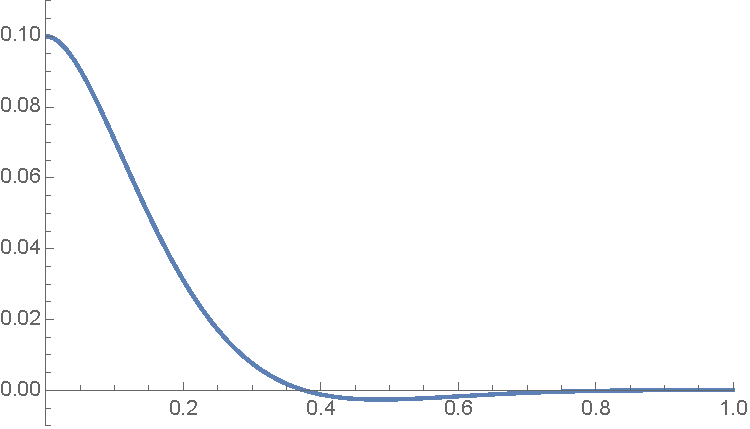
\includegraphics{p17plot.pdf}

The mass is placed $0.1$ $m$ from its equilibrium position. After releasing it, it returns to its equilibrium position within $0.4$ $s$ and passes its equilibrium position a little bit. Then, it returns to its equilibrium position slowly, and stops at the equilibrium position. 

\end{solution}

\item Solve $y^{IV} - 6y^{III} + 13y^{II} + 24y^I + 36 = 0$ subject to the conditions that $y(0) = 0, \: y^I(0) = 1, \: y(1) = 0, \: y^I(1) = -10$.  This is known as a boundary value problem because rather than specifying conditions on y at the start of the interval in x, we specify conditions at both ends. Since the equation has four derivatives, four boundary conditions are necessary. Hints: even though this is a high order equation, you can still write down its characteristic equation. To solve for the coefficients in the general solution, you will want to plug in the given boundary conditions to obtain four equations. Use a computer to solve these.

\begin{solution}

We can start our solution by guessing that $y = e^{\lambda t}$ is a solution and substituting in.  The $n$th derivative of $y$, $y^n = \lambda^ne^{\lambda t}$.  Therefore, after substitution and cancellation, we get the characteristic equation
\[
\lambda^4 - 6\lambda^3 + 13\lambda^2 - 24\lambda + 36 = 0
\]

A brief consultation with Mathematica ...
\begin{verbatim}
In[1]:= Solve[y^4 - 6y^3 + 13y^2 - 24y + 36 == 0, y]
Out[1]= {{y -> -2 I}, {y -> 2 I}, {y -> 3}, {y -> 3}}
\end{verbatim}
tells us that three solutions are $e^{i2t}$, $e^{-i2t}$, and $e^{3t}$.  However, there are two $3$s, so we need to try something else for the fourth solution.  In this case, we guess that it's of the form $y = v(t)e^{3t}$.  For this, we need the derivatives which are:
\begin{align*}
y &= ve^{3t} \\
y^I &= v'e^{3t} + 3ve^{3t} = e^{3t}(3v + v') \\
y^{II} &= e^{3t}(3v' + v'') + 3e^{3t}(3v + v') = e^{3t}(9v + 6v' + v'') \\
y^{III} &= e^{3t}(9v' + 6v'' + v''') + 3e^{3t}(9v + 6v' + v'') = e^{3t}(27v + 27v' + 9v'' + v''') \\
y^{IV} &= e^{3t}(27v' + 27v'' + 9v''' + v'''') + 3e^{3t}(27v + 27v' + 9v'' + v''')\\
&= e^{3t}(81v + 108v' + 54v'' + 12v'' + v'''')
\end{align*}

With these derived, we can plug into the equation and get this monstrosity:
\begin{multline*}
e^{3t}(81v + 108v' + 54v'' + 12v'' + v'''') - 6e^{3t}(27v + 27v' + 9v'' + v''') + \\
13e^{3t}(9v + 6v' + v'') - 24e^{3t}(3v + v') + 36ve^{3t} = 0
\end{multline*}

After some distribution and rearrangement for readability, we get the following

\begin{align*}
&81v + \:\:\:\:\:\: 108v' + 54v'' + 12v''' + v''''  +  \\
&-162v - 162v' - 54v'' - 6v'''  +  \\
&117v + \:\:\: 78v' + \:\:\: 13v'' + \\
&-72v - \: 24v' + \\
&36v \\
\end{align*}

which simplifies to
\[
13v'' + 6v''' + v'''' = 0
\]


Since each term is multiplied by at least a factor of $v''$, we can integrate both sides of the equation. This gives us

\begin{equation}
v'' + 6v' + 13v = c_{1}t + c_{2}
\end{equation}

Now this is an inhomogeneous linear equation, so we solve it by breaking it into the homogeneous and particular solutions.

For the homogeneous solution,

\[
v'' + 6v' + 13v = 0
\]

yields roots of $-3 \pm 2i$. To solve the inhomogeneous equation

\[
v_{p}'' + 6v_{p}' + 13v_{p} = c_{1} + c_{2}
\]

we set up equations for $v_{p}$:

\[
v_{p} = At + B
\]
\[
v_{p}' = A
\]
\[
v_{p}'' = 0
\]

Substituting these into the original equation gives us

\[
v_{p}'' + 6v_{p}' + 13v_{p} = 6A + 13At + 13B = c_{1}t + c_{2}
\]

We can now solve for these constants.
\[
c_{1} = 13A
\]
\[
c_{2} = 6A + 13B
\]

This gives us $A = \frac{c_{1}}{13} = c_{3}$ and $B = \frac{13c_{2}-6c_{1}}{169} = c_{4}$. 

Now we can create a solution for $y(t)$ using linear combinations of our solutions! The solutions are $e^{2it}, e^{-2it}, e^{3t},$ and $te^{3t}$. For the sake of clarity and ease of explanation from this point on, we are resetting our constants (since they are all just constants anyway!).

\begin{equation}
y(t) = c_{1} t e^{3t} + c_{2}e^{3t} + ae^{2it} + be^{-2it}
\end{equation}

To simplify things, we are going to put the imaginary exponentials in terms of $\sin$ and $\cos$ using Euler's formula. Let $c_{3} = a + b$ and $c_{4} = ai - bi$.

\begin{equation}
y(t) = c_{1} t e^{3t} + c_{2}e^{3t} + c_{3}\cos{(2t)} + c_{4}\sin{(2t)}
\end{equation}

We can also find the derivative of this equation.

\begin{equation}
y'(t) = 3 c_{1} t e^{3t} + c_{1}e^{3t} + 3c_{2}e^{3t} - 2 c_{3}\sin{(2t)} + 2c_{4}\cos{(2t)} 
\end{equation}

\[
y'(t) = 3 c_{1} t e^{3t} + (c_{1} + 3c_{2})e^{3t} - 2 c_{3}\sin{(2t)} + 2c_{4}\cos{(2t)}
\]

Now we use our boundary conditions to set up a system of equations that will allow us to solve for our four constants.

\[
y(0) = 0 = c_{2} + c_{3}
\]
\[
y(1) = 0 = c_{1}e^{3} + c_{2}e^{3} + c_{3}\cos{(2)} + c_{4}\sin{(2)}
\]
\[
y'(0) = 1 = c_{1} + 3c_{2} + 2c_{4}
\]
\[
y'(1) = -10 = 3 c_{1} e^{3} + (c_{1} + 3c_{2})e^{3} - 2 c_{3}\sin{(2)} + 2c_{4}\cos{(2)}
\]

We solve this system of equations using fancy software, which gives us some absurd constants. (Note: in this image, $a$ corresponds to $c_{1}$, $b$ corresponds to $c_{2}$, etc.)

\begin{center}
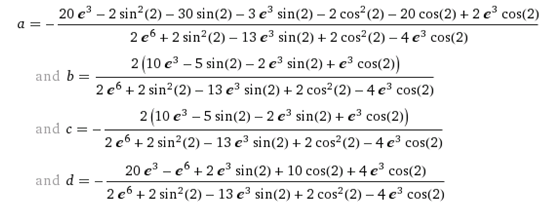
\includegraphics{constants.png}
\end{center}

Because typing that out would be a bear, our final solution is going to be an equation using references to those constants:

\begin{equation}
y(t) = a t e^{3t} + be^{3t} + c\cos{(2t)} + d\sin{(2t)}
\end{equation}

\end{solution}

\item Consider the Van der Pol Oscillator, $m\ddot{x} + \mu(x^2 - 1)\dot{x} + kx = 0$.  Note that this is a nonlinear equation.  Here, $m, \mu, k > 0$.
\begin{enumerate}
\item Comparing this equation to the usual second-order (linear) oscillator equation, $m\ddot{x} + \mu\dot{x} + kx = 0$, discuss the effect of the nonlinear term.  Hint: think about the sign of each part of the parenthetical  terms, and interpret each one of these terms (and then, their combination) in terms of friction.
\item Set $m = 1, k = !, \mu = 1$.  Solve the equation numerically for $x(0) = 0.1, \dot{x}(0) = 0$ for $0 \leq t \leq 200$.  Then repeat for $x(0) = 6, \dot{x}(0) = 6$.  To show your solutions, plot them in the phase plane, which means you plot $x$ on the horizontal and $\dot{x}$ on the vertical.  Plot both solutions on the same graph and describe what you see.
\end{enumerate}

\begin{solution}
\begin{parts}
\part
The Van der Pol oscillator has an exponential term to combine with $\mu$.  Thinking about this in terms of friction means that there will be exponential growth of the correcting force as the spring stretches, so it will start much lower than a linear spring and quickly exceed the linear spring's.
\part
\begin{verbatim}
function [t, x] = vanderpol
%Solves the ODE xddot = -(x1^2-1)*x2 - x1 and gives output as [t,x1,x2]
 
%Set start and end times
t0 = 0;
tf = 200;
 
%Solve the ODE
[t,x] = ode45(@F, [t0, tf], [6, 6], []);
end

function xp = F(t, x)
xp = zeros(2,1);
xp(1) = x(2);
xp(2) = -1*(x(1)^2 - 1)*x(2) - x(1);
end
\end{verbatim}

\begin{center}
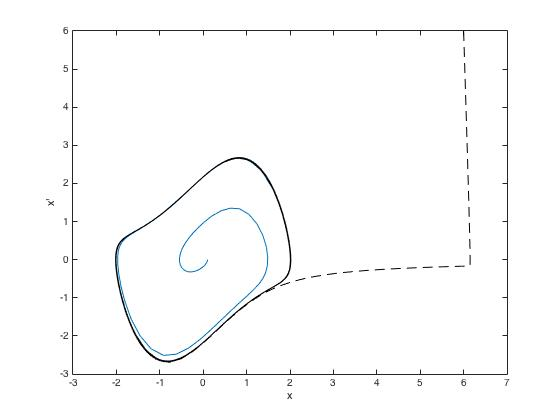
\includegraphics[width=0.6\textwidth]{van_der_pol_19b.jpg}
\end{center}

\end{parts}
\end{solution}

\item A building consists of two floors. The first floor is attached rigidly to the ground and the second floor is of mass $m = 104 kg$. The elastic frame of the building acts as a Hookean (linear) spring that resists horizontal displacements of the second floor. It requires a horizontal force of $5\times 10^7 kg \cdot m/s^2$
\begin{enumerate}
\item Find the general solution of the differential equation describing the displacement of the second floor.
\item What is the (natural) frequency of oscillations of the second floor?
\item Assume that in an earthquake, the ground oscillates horizontally with amplitude $A_0$ and frequency $\omega$ (not equal to the natural frequency) resulting in an external force $F(t) =m A_0 \omega^2\sin(\omega t)$ on the second floor.  Find the solution of the differential equation describing this situation, assuming that the second floor is initially at rest and at zero displacement.
\item Explain (in words) the motion described by the solution you just found, making sure to comment on if/when it is periodic. (If you don’t know what I am talking about, a link such as \href{https://mathblag.wordpress.com/2013/09/01/sums-of-periodic-functions/}{this} might help you.)
\item The solution you derived in part (c) does not apply in one special case. Suppose that the earthquake’s frequency $\omega$ is equal to the natural frequency that you found in part (b). Re-derive the solution for $x(t)$ in this case.
\item Explain (in words) the motion described by the solution you just found, and compare it to the previous case. Hint: the phenomenon you are seeing is called “resonance.”
\end{enumerate}
\begin{solution}
\begin{enumerate}
\item Starting with $F = kx$, we can plug in $x = 0.5m$ and $F = 5\times 10^7$ to solve for $k$ which turns out to be $10^8$.  Then we can plug the force equation into Newton's equations to find that
\[
kx = m\frac{d^2x}{dt^2}
\]
By guessing that $x = e^{\lambda t}$, we can find that $\lambda^2 = 10^4$, making $\lambda = \pm 100$, so the general solution is
\[
y = C_1e^{100t} + C_2e^{-100t}
\]

\item The natural frequency of a function is $\Xi/2\pi$ where $\Xi$ is found as $\sin{(\Xi x)}$ or $\cos{(\Xi x)}$.  We can take our general solution from before and apply Euler's formula to find that:

\[
y = C_1e^{100t} + C_2e^{-100t} = (C_1 + C_2)\cos(100t) + (C_1 - C_2)i\sin{(100t)}
\]

so the frequency is $100/2\pi = 50/\pi \approx 15.92$

\item Here, we have a non-homogeneous equation.  The homogeneous parts will still act as solutions, but we need to find the particular solution.  Our equation goes from $kx - ma = 0$ to $kx - ma = m A_0 \omega^2\sin(\omega t)$.  Because of this, we can guess that our particular solution will be of the form $A\cos(\omega t) + B\sin(\omega t)$.  First we start with the derivatives:
\begin{align*}
x &= A\cos{(\omega t)} + B\sin{(\omega t)}\\
\dot{x} &= \omega B\cos{(\omega t)} - \omega A\sin{(\omega t)}\\
\ddot{x} &= -\left( \omega^2B\sin{(\omega t)} + \omega^2A\cos{(\omega t)} \right)
\end{align*}

From here, we can plug these into our equation, which gives us
\[
\frac{k}{m}\left(A\cos{(\omega t)} + B\sin{(\omega t)}\right) + \omega^2B\sin{(\omega t)} + \omega^2A\cos{(\omega t)} = A_0 \omega^2\sin{(\omega t)}
\]

From here, we can separate this into two different equations - one with all the $\cos$ terms set to zero and one with all the $\sin$, set to $A_0 \omega^2\sin{(\omega t)}$.  When we do this, we get:

\begin{align*}
\frac{k}{m}A\cos{(\omega t)} + \omega^2 A\cos{(\omega t)} &= 0 \\
\frac{k}{m}B\sin{(\omega t)} + \omega^2B\sin{(\omega t)} &= A_0 \omega^2\sin{(\omega t)}
\end{align*}

Just looking at these equations, one can see that $A = 0$, and with some minor algebra, we find that $\displaystyle B = \frac{A_0\omega^2m}{\omega^2m + k}$

From here, we have a general equation for $x$ from which we can find coefficients.  Our general solution and its derivative is
\begin{align*}
x &= C_1(\cos(100t) + i\sin(100t)) + C_2(\cos(100t - i\sin(100t)) + \frac{A_0\omega^2m}{\omega^2m + k}\sin{\omega t}\\
x &= (C_1 + C_2)\cos{(100t)} + (C_1 - C_2)o\sin{(100t)} + \frac{A_0\omega^2m}{\omega^2m + k}\sin{\omega t}\\
\dot{x} &= -100(C_1 + C_2)\sin{(100t)} + 100i(C_1 - C_2)\cos{(100t)} + \frac{A_0\omega^2m}{\omega^2m + k}\cos{\omega t}
\end{align*}

We know that $x(0) = 0$ and $\dot{x}(0) = 0$, which leads us the equations:

\begin{align*}
x(0) &= C_1 + C_2 = 0 \Rightarrow C_1 = -C_2 \\
\dot{x}(0) &= 100i(C_1 - C_2) + \frac{A_0\omega^2m}{\omega^2m + k} = 0
\end{align*}

For the second equation, we can substitute $C_1$ for $-C_2$ and find that 
\[
200iC_1 = -\frac{A_0\omega^3m}{\omega^2m + k} \Rightarrow C_1 = -\frac{A_0\omega^3m}{200i(\omega^2m + k)}
\]

Plugging that in for $C_1$ and its negative for $C_2$, we find that 
\begin{align*}
x &= \frac{A_0\omega^3m}{100(\omega^2m + k)}\sin(100t) + \frac{A_0\omega^2m}{\omega^2m + k}\sin{(\omega t)} \\
&= \frac{A_0\omega^3 10^4}{100(\omega^2 10^4 + 10^8)}\sin(100t) + \frac{A_0\omega^2 10^4}{\omega^2 10^4 + 10^8}\sin{(\omega t)} \\
&= \frac{A_0 \omega^2 m}{(\omega^2 m + k)}(\frac{\omega}{100}\sin{(100t)} + \sin{(\omega t)})
\end{align*}

\item The motion of this building is only periodic when the periods of the two $\sin$ terms are multiples of each other. Since the period of $\sin{(100t)}$ is $\frac{2\pi}{100} = \frac{\pi}{50}$, $\omega$ must be a multiple of 100 to make the function periodic. The period of the term $\sin{(\omega t)}$ will be a multiple of $\frac{\pi}{50}$. When $\omega$ is not a multiple of $100$, the sum of these periodic terms is not periodic. For example, compare an example of what motion of the building could look like when $\omega = 200$ (the left graph) versus when $\omega = 175$ (the right graph). 

\begin{center}
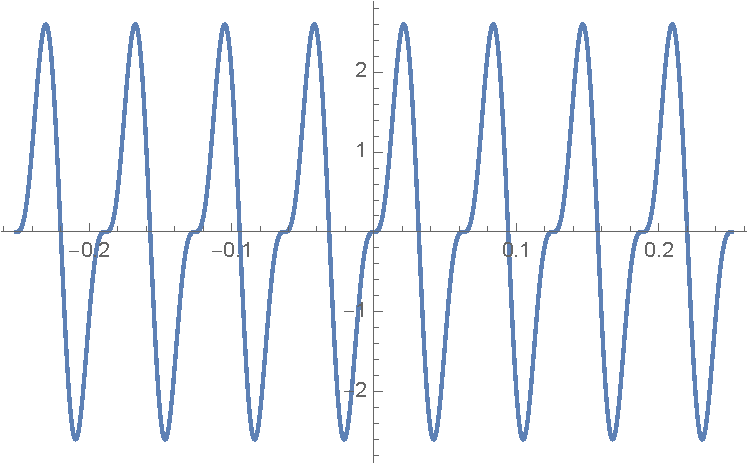
\includegraphics[width=0.3\textwidth]{yay_200.pdf}
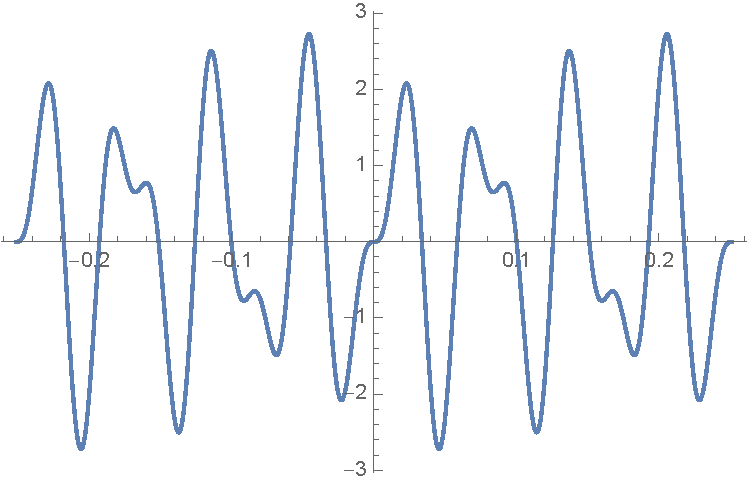
\includegraphics[width=0.3\textwidth]{yay_.pdf}
\end{center}

\item If we substitute in our building's frequency - $50/\pi$ - for $\omega$, (and add in all the constants that have been left as variables so far) we get the equation:

\[
x = \frac{A_0 (50/\pi)^2 10^4}{((50/\pi)^2 10^4 + 10^8)}\left(\frac{50/\pi}{100}\sin{(100t)} + \sin{(50/\pi t)}\right)
\]

\item This solution again has two $\sin$ terms. The first has a period of $\frac{2\pi}{\frac{50}{100\pi}} = 4\pi^{2}$. The second, using our natural frequency of $\omega = \frac{50}{\pi}$, has a period of $\frac{2\pi}{\frac{50}{\pi}} = \frac{\pi^{2}}{25}$. Instead of giving a curve in which it is easy to determine which parts of the curve come from which component of the function, these $\sin$ functions combine to give a more complex periodic function with a larger amplitude than would be expected if the two frequencies were not resonant.
\end{enumerate}


\end{solution}
\end{questions}
\end{document}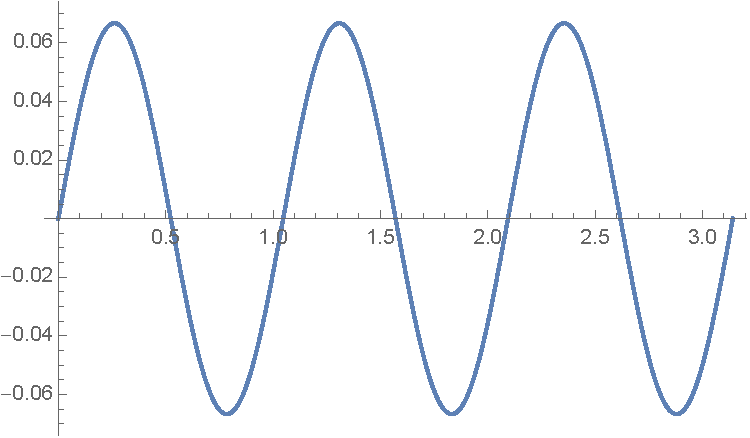
\includegraphics{p16plot.pdf}